\graphicspath{{../Graphics/Cpt1-Charactz/}}

Antes de abordar el estudio de la dinámica no lineal del láser de semiconductor de modo discreto se ha realizado la simulación del láser en solitario, sin inyección de luz del láser esclavo ($P_{Iny} = 0$).Se han realizado simulaciones para el láser tanto en corriente continua (CW de sus siglas en inglés) con en Gain-Switching, comparando los resultados con los obtenidos experimentalmente en condiciones similares \cite{Chaves19}.

	\addtocontents{toc}{\vspace{0.1cm}}
	\section{Láser en corriente continua}

		Para poder realizar las simulaciones en CW se ha trabajado con una corriente igual a la corriente de polarizaci'on ($I(t) = I_{Bias}$), tomando $V_{RF}$, y as'i la amplitud de modulaci'on.

		\addtocontents{toc}{\vspace{0.1cm}}
		\subsection{Espectros de emisión}

		
				% Img:spectrosCW {Img:spectrosCW:sim, Img:spectrosCW:exp}
				\begin{figure}[H]
					\centering
					\begin{subfigure}{0.45\textwidth}
						\centering
						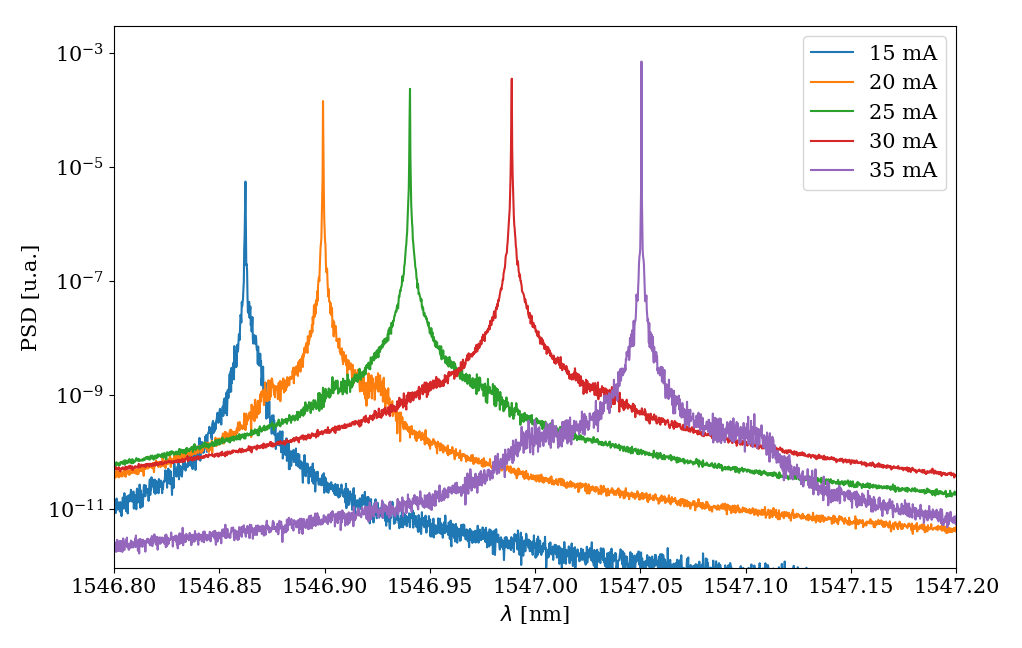
\includegraphics[width=1.0\linewidth, height=6cm]{Espectros.png}
						\caption{\label{Img:spectrosCW:sim}Espectros ópticos obtenidos mediante simulación.}
					\end{subfigure}
					\begin{subfigure}{0.45\textwidth}
						\centering
						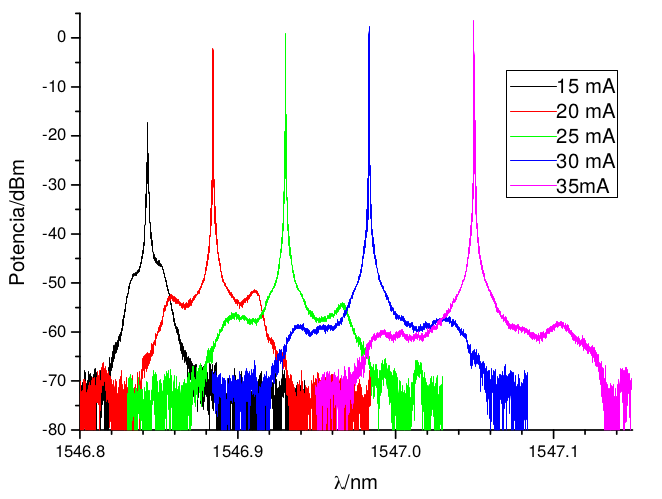
\includegraphics[width=1.0\linewidth, height=6cm]{../Chaves/OFC-GS/espectros_continua.png}
						\caption{\label{Img:spectrosCW:exp}Espectros ópticos obtenidos experimentalmente.}	
					\end{subfigure}
					\caption{\label{Img:spectrosCW}Espectros ópticos del DML para diferentes corrientes de polarización $I_{Bias}$ obtenidos mediante simulación (izquierda \ref{Img:spectrosCW:sim}) y esperimentalmente (derecha, \ref{Img:spectrosCW:exp}).}
				\end{figure}
 
 				% tab:lambdas
				\begin{table}[H]
					\centering
					\begin{tabular}{c c c}
						\hline
						$I_{Bias}$ & $\lambda_{sim}$ & $\lambda_{exp}$ \\\hline 
						15 & 1546.86 & 1546.84 \\
						20 & 1546.90 & 1546.88 \\
						25 & 1546.94 & 1546.93 \\
						30 & 1546.99 & 1546.98 \\
						35 & 1547.05 & 1547.05 \\\hline
					\end{tabular}
					\caption{\label{tab:lambdas}Longitud de onda de las lineas de emisión del DML en función de la $I_{Bias}$ obtenidas de la figura \ref{Img:spectrosCW}. Se muestran los valores experimentales $\lambda_{exp}$ obtenidos de la gráfica \ref{Img:spectrosCW:exp} con un error de $\delta\lambda_{exp} = 0.02$, y los valores obtenidos de la simulación de la gráfica \ref{Img:spectrosCW:sim}.}
				\end{table}

			Las longitudes de onda de la tabla \ref{tab:lambdas} muestran una gran concordancia entre los resultados esperimentales y los obtenidos a partir de la simulación del DML. 
	
		\addtocontents{toc}{\vspace{0.1cm}}
		\subsection{Transitorio}

			Pese a que la zona de estudio del DML comienza 
				
				% Img:transitorio
				\begin{figure}[H]
					\centering
					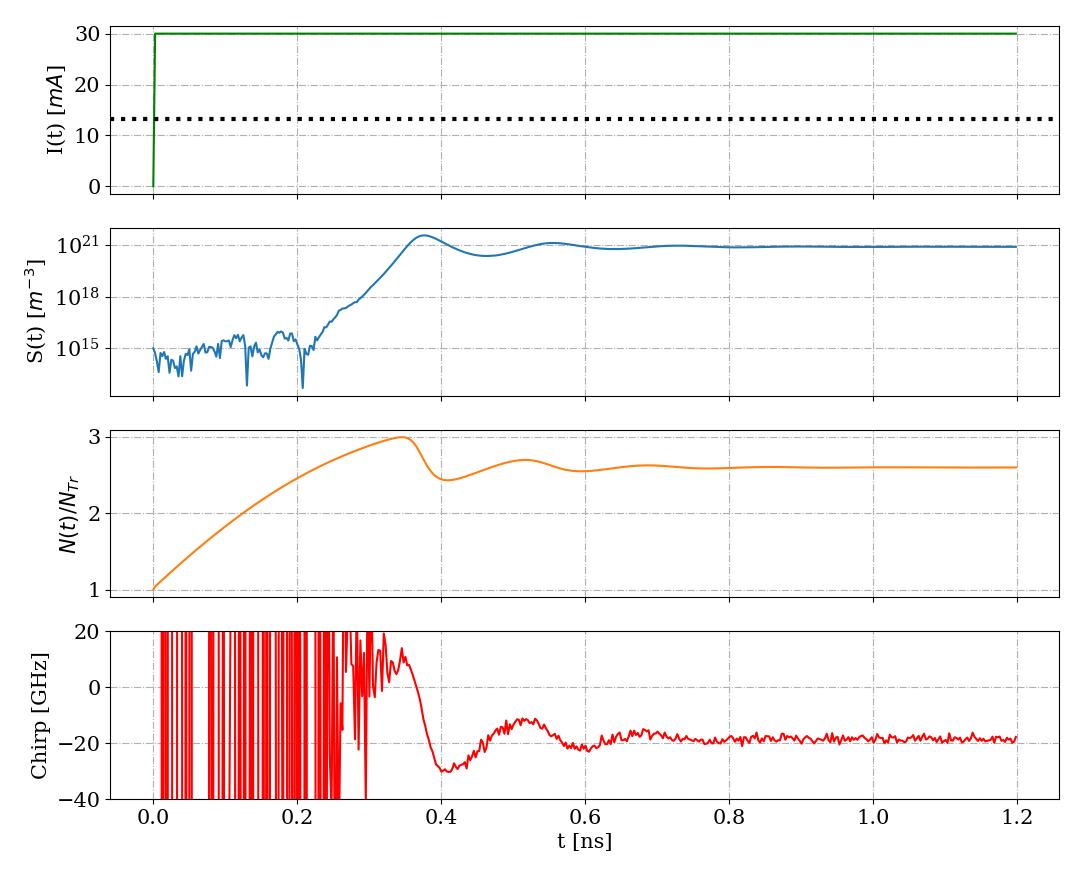
\includegraphics[width=0.7\linewidth]{transitorio.png}
					\caption{\label{Img:transitorio}Transitorio}	
				\end{figure}
				kkk

	\addtocontents{toc}{\vspace{0.1cm}}
	\section{OFC (Gain-Switching)}

		\addtocontents{toc}{\vspace{0.1cm}}
		\subsection{Efecto de la amplitud de modulación a altas frecuencias}

				% Img:rateEquations
				\begin{figure}[H]
					\centering
					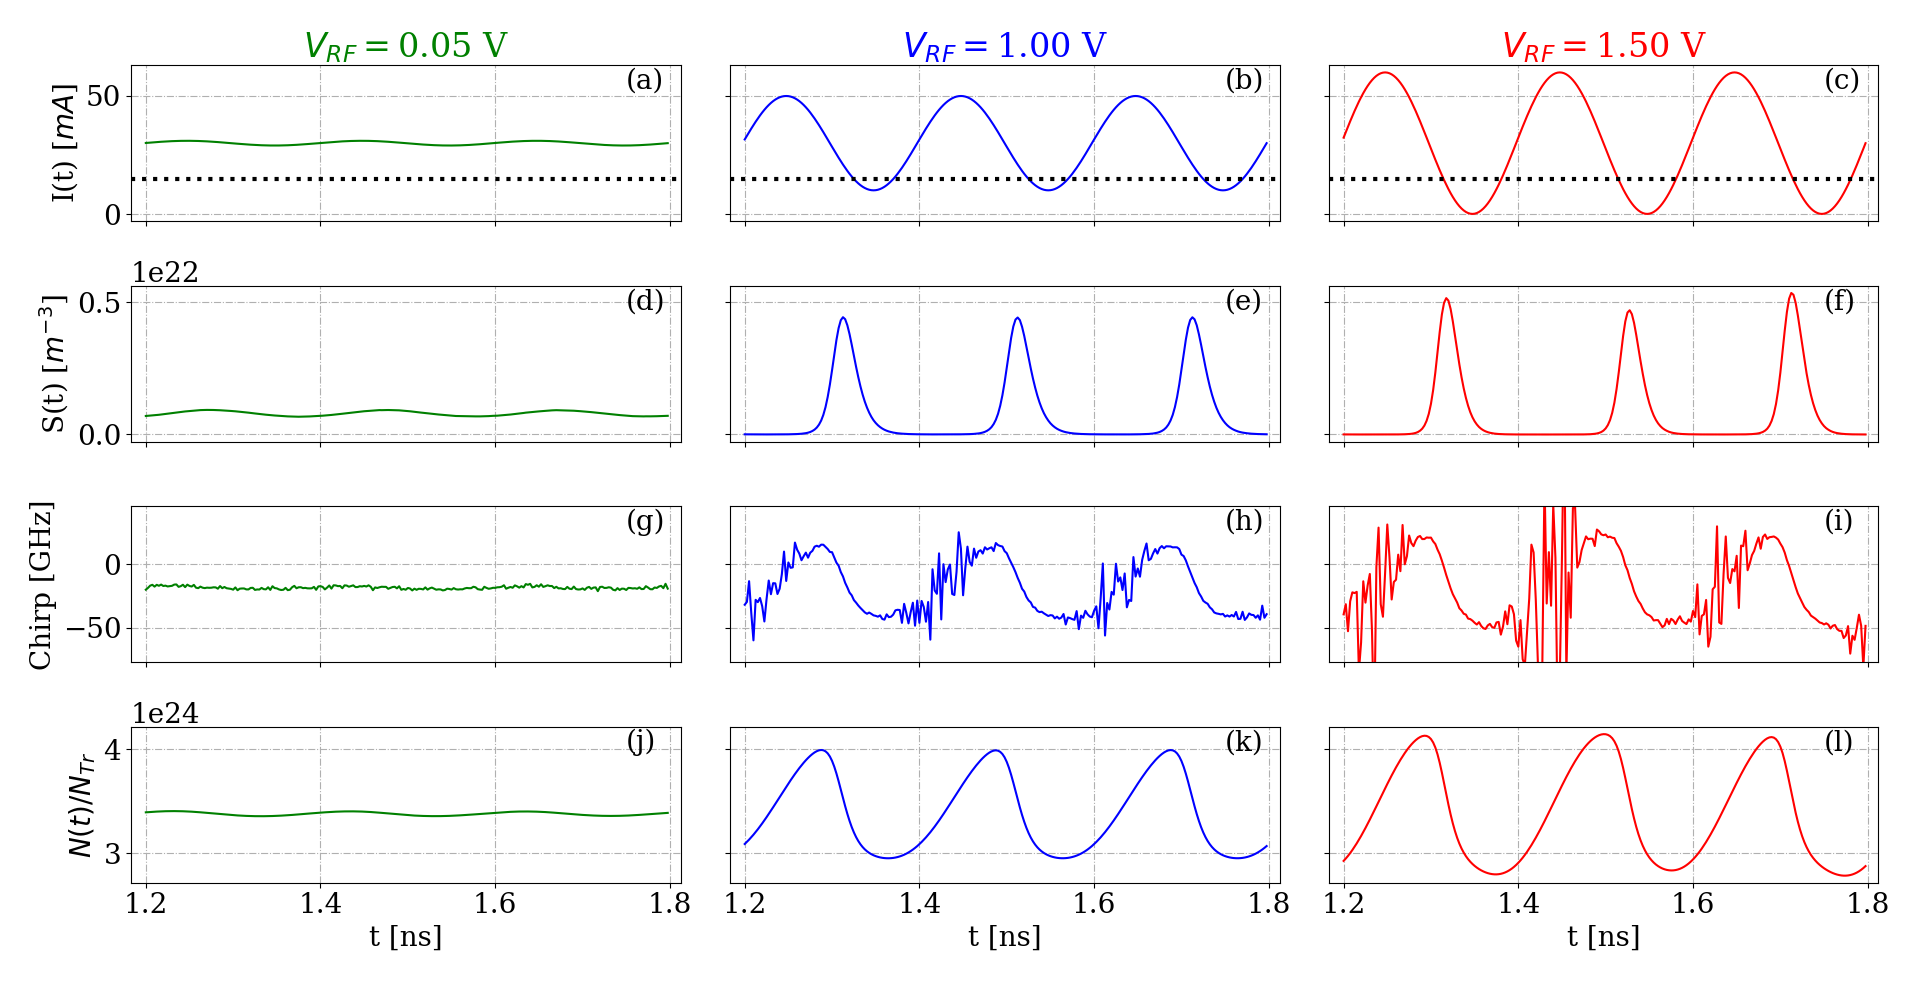
\includegraphics[width=1.0\linewidth]{rateEquations.png}
					\caption{\label{Img:rateEquations}RateEquations}	
				\end{figure}

				% Img:PSD
				\begin{figure}[H]
					\centering
					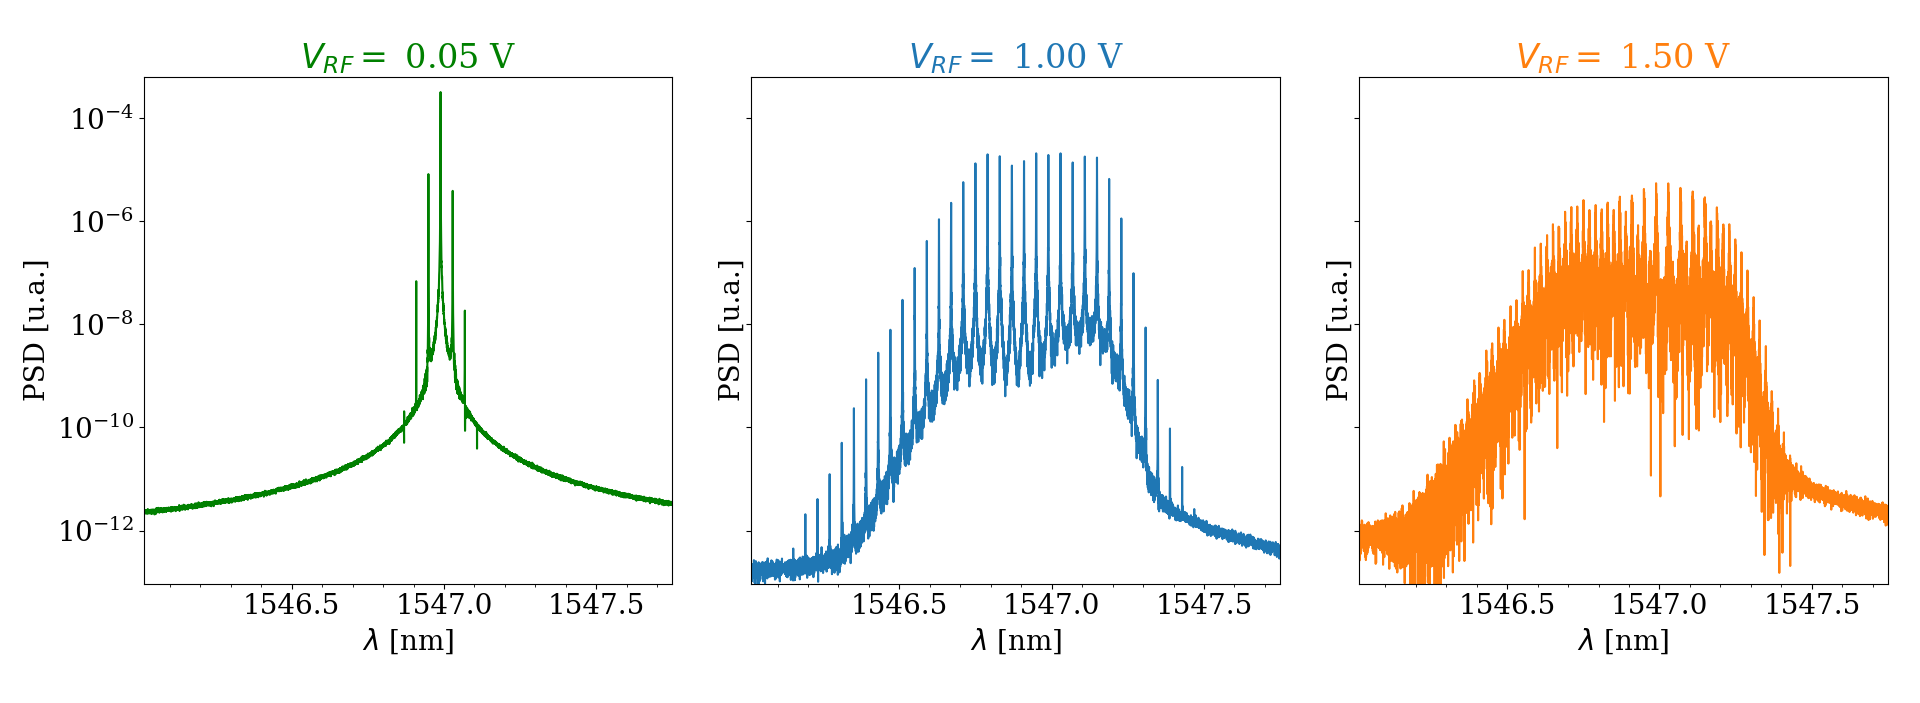
\includegraphics[width=1.0\linewidth]{PSD.png}
					\caption{\label{Img:PSD}PSD}	
				\end{figure}

				% Img:current
				\begin{figure}[H]
					\centering
					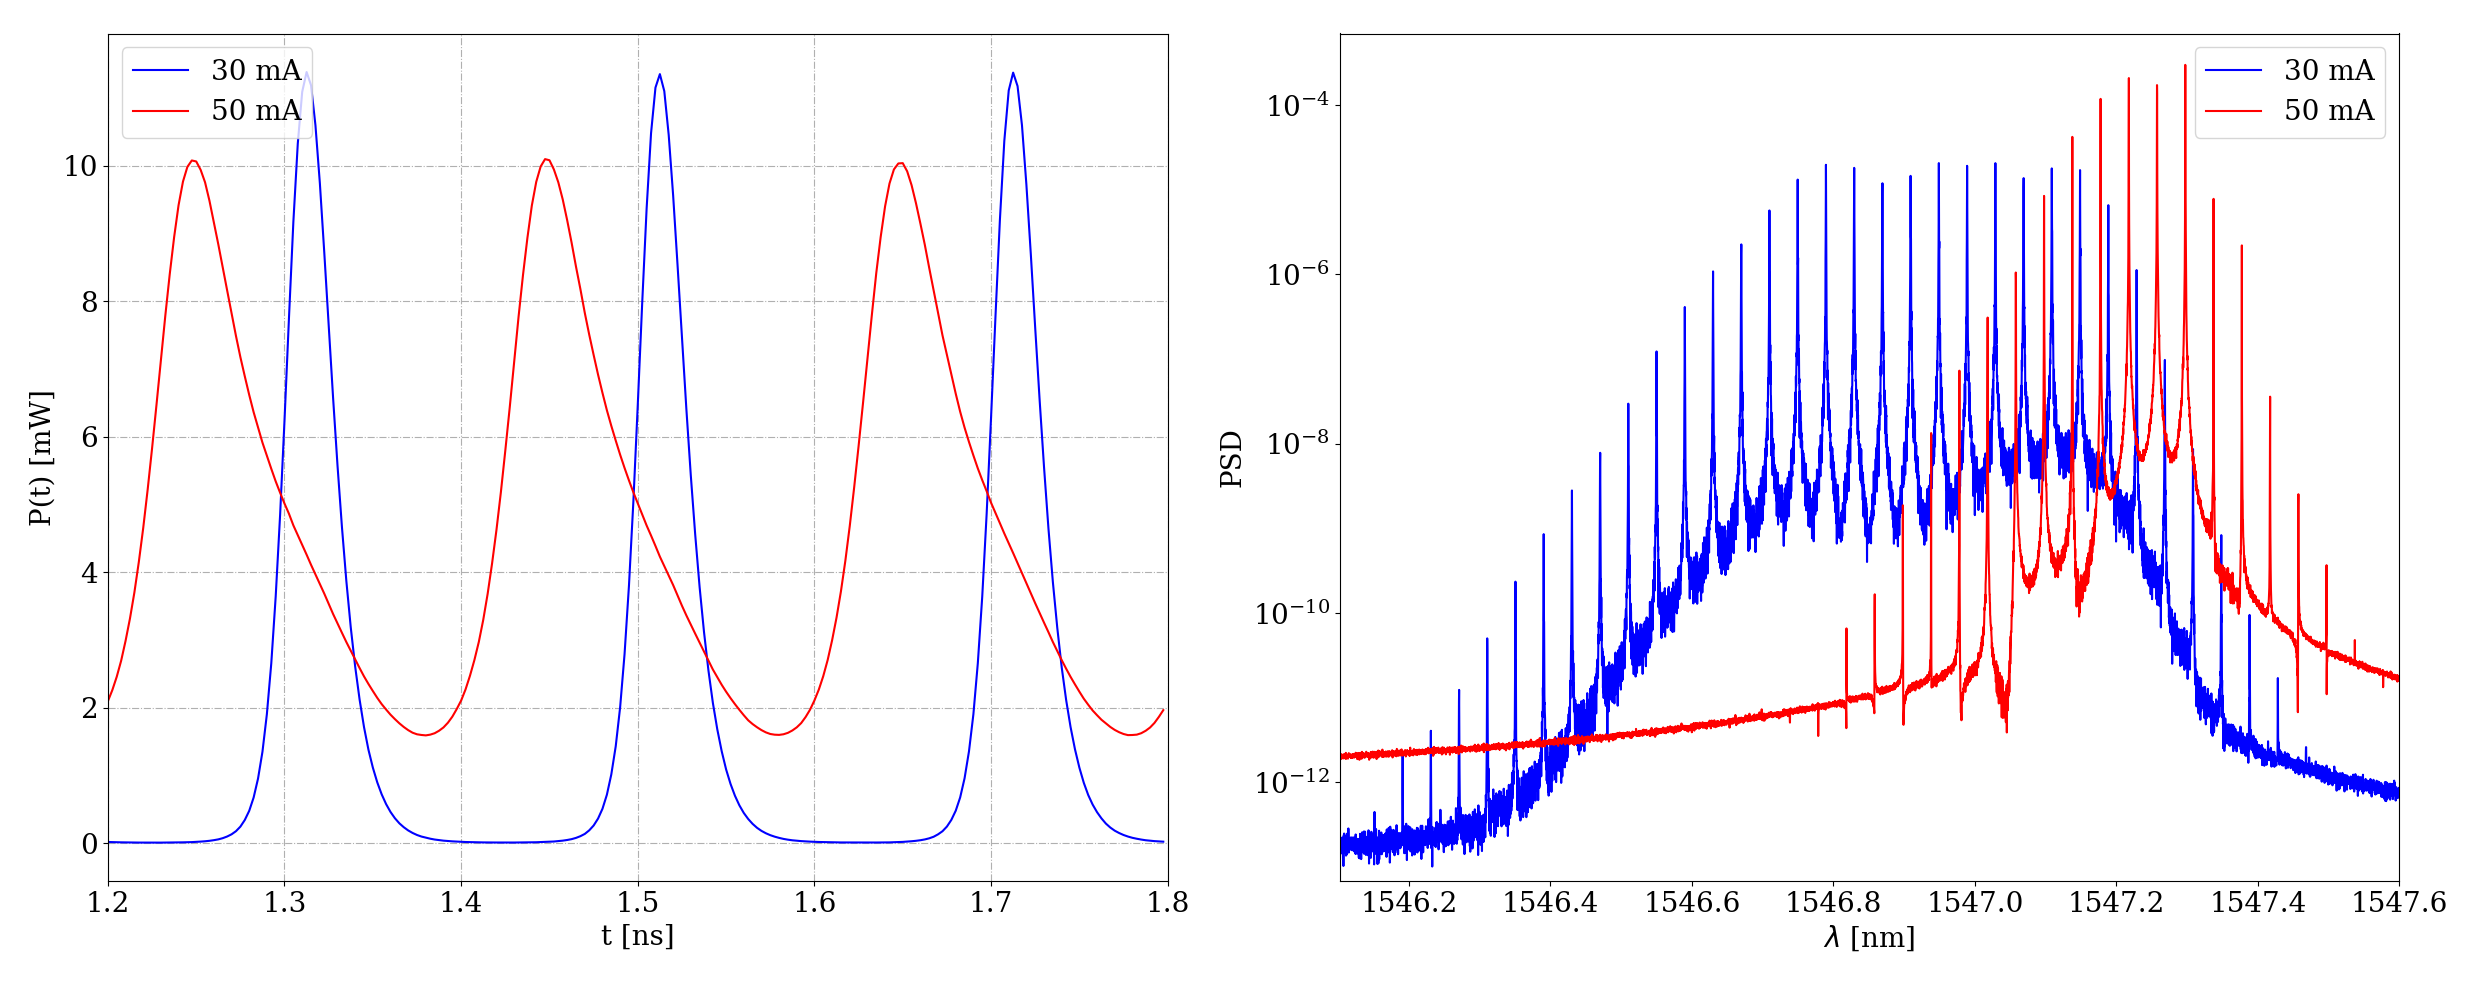
\includegraphics[width=1.0\linewidth]{current.png}
					\caption{\label{Img:current}Current}	
				\end{figure}

		\addtocontents{toc}{\vspace{0.1cm}}
		\subsection{Efecto de la amplitud de modulación a bajas frecuencias}

				% Img:500
				\begin{figure}[H]
					\centering
					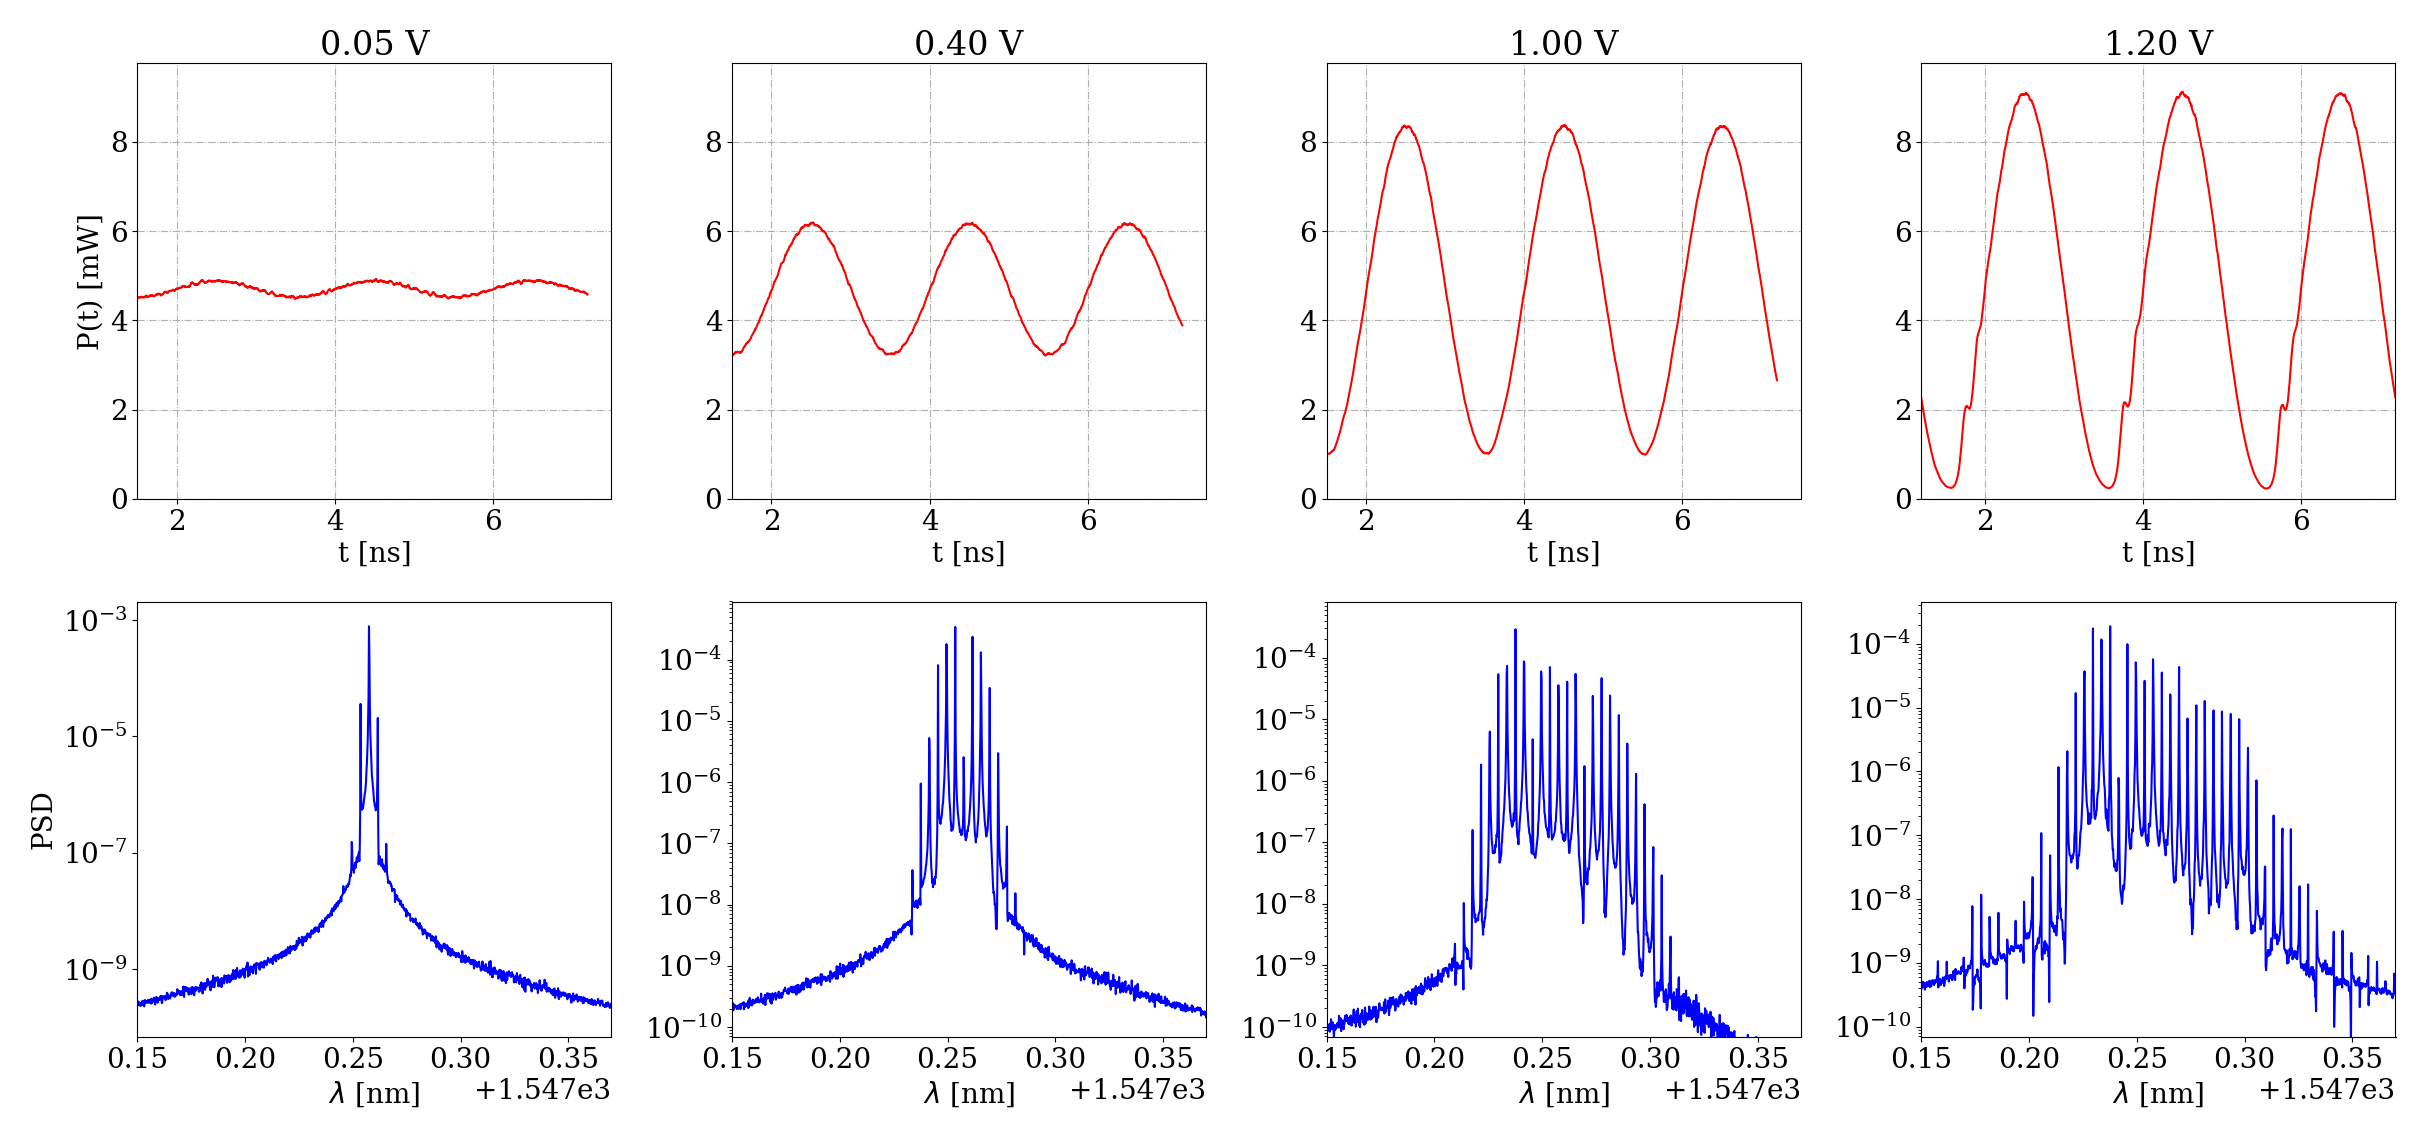
\includegraphics[width=1.0\linewidth]{500.png}
					\caption{\label{Img:500}500}	
				\end{figure}

				% Img:500mhz
				\begin{figure}[H]
					\centering
					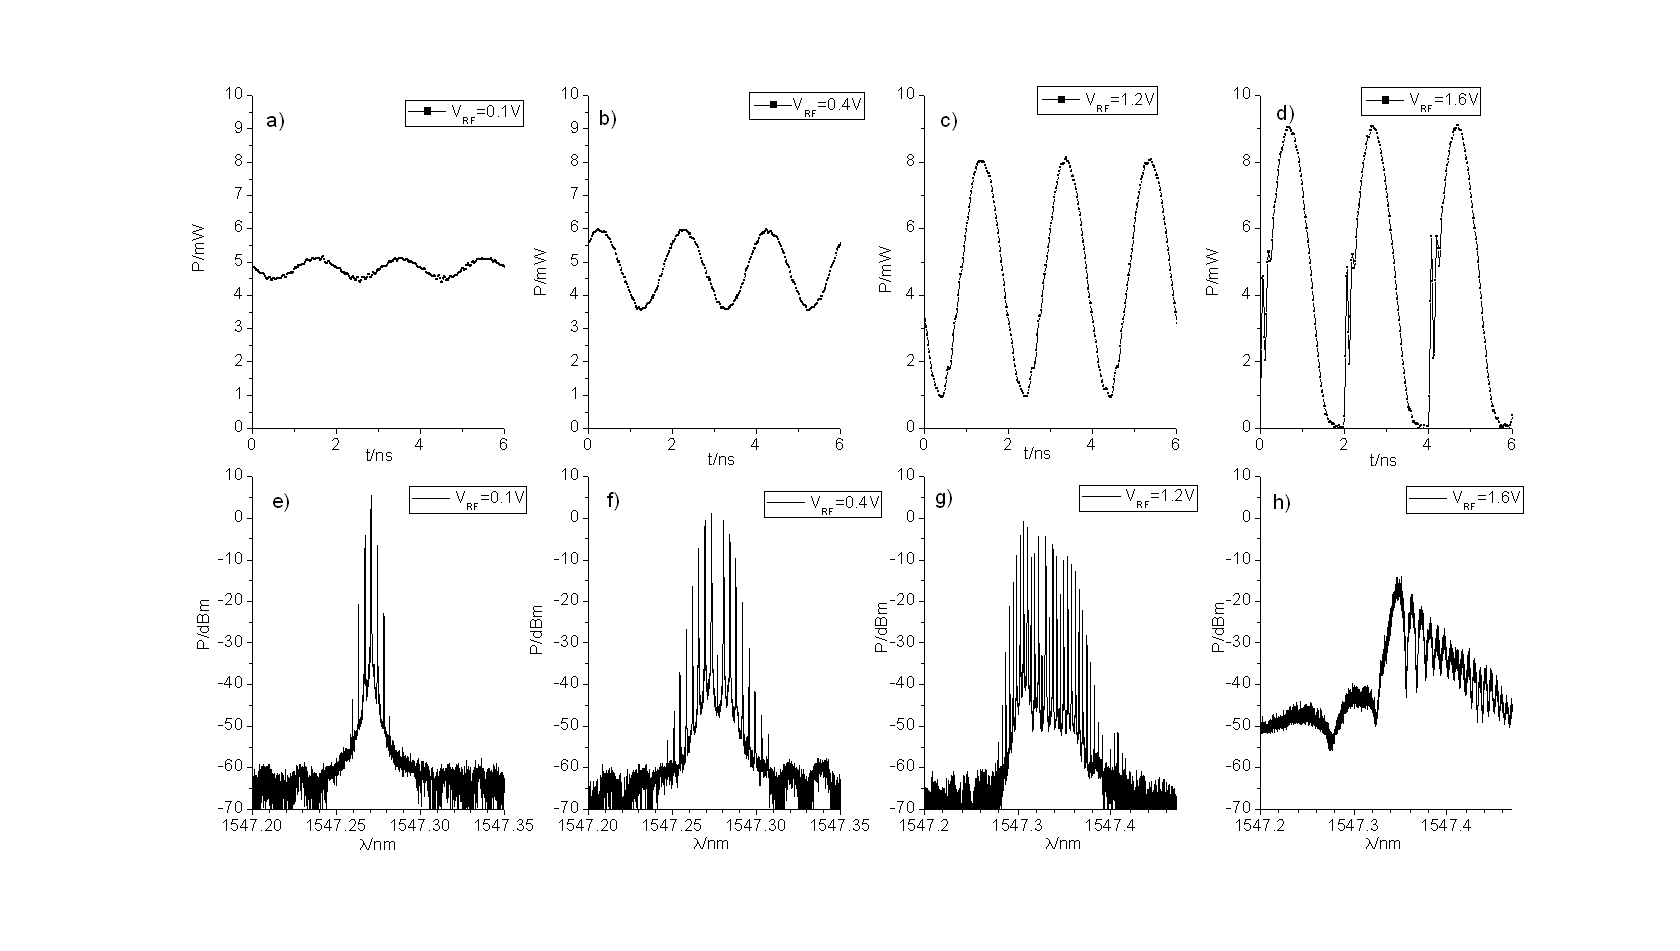
\includegraphics[width=1.0\linewidth]{../Chaves/OFC-GS/500mhz.png}
					\caption{\label{Img:500mhz}500mhz}	
				\end{figure}
